\chapter{Demo}
Demo link\footnote{Only available for certain time}: \url{https://bajgain.tech}\\

\section{Program Tabs, screenshots and info}
Program has theme selection, so screenshots are diffrent.\\
\subsection{Start Screen}
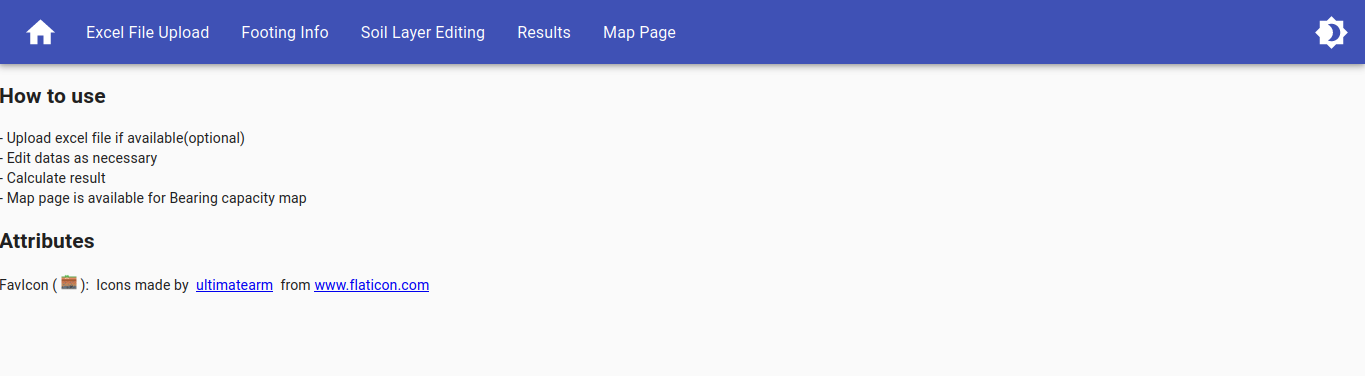
\includegraphics[width=\linewidth,keepaspectratio]{../proj/soilbearing/media/images/index.png}
General info about program\\

\subsection{Upload Tab}
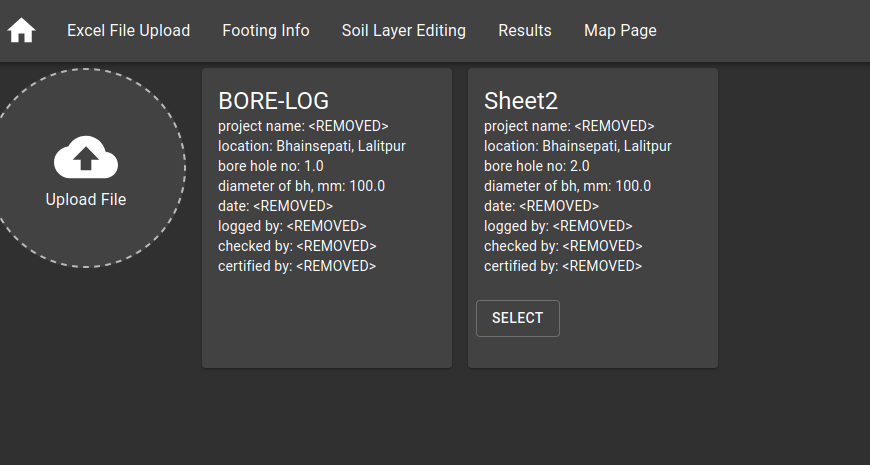
\includegraphics[width=\linewidth,keepaspectratio]{../proj/soilbearing/media/images/fileInfo.png}
Upload the excel file. (either .xls, or .xlsx)\\
If more than one sheet is available in file then sheet selection option.\\
\begin{itemize}
\item Click and select, or\\
\item drag and drop\\
\end{itemize}

\subsection{Footing info Tab}
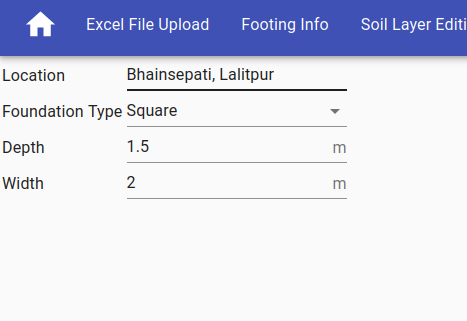
\includegraphics[width=\linewidth,keepaspectratio]{../proj/soilbearing/media/images/footing_info.png}
Basic footing info,\\

\subsection{Edit Tab}
There are 2 modes:-\\
\subsubsection{Edit Mode}
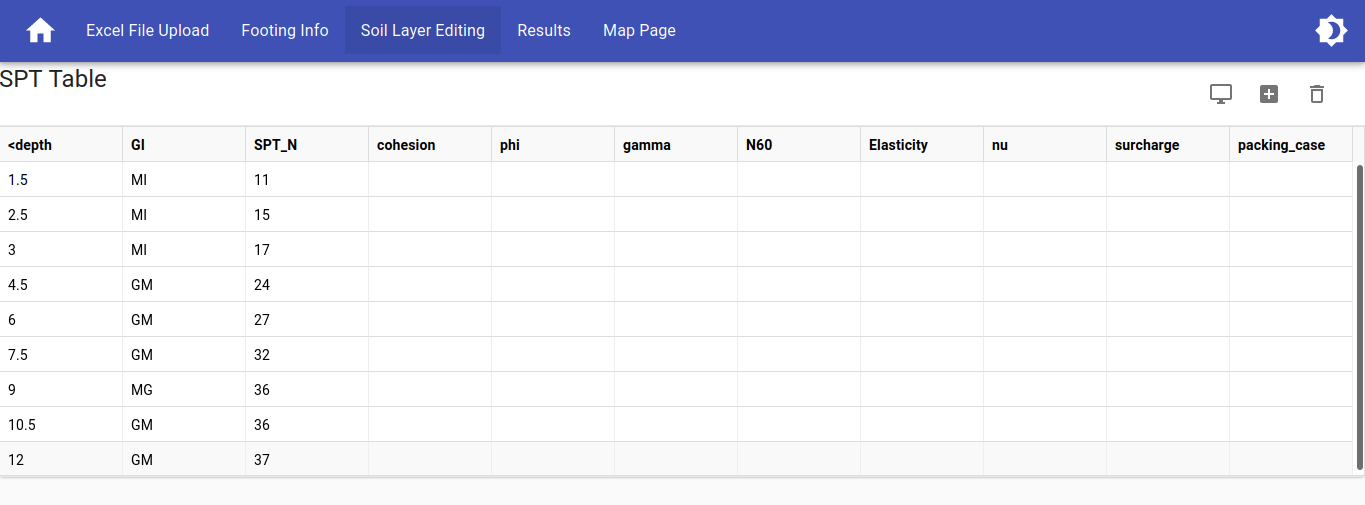
\includegraphics[width=\linewidth,keepaspectratio]{../proj/soilbearing/media/images/edit_mode.png}
Actual editing\\

\subsubsection{Preview Mode}
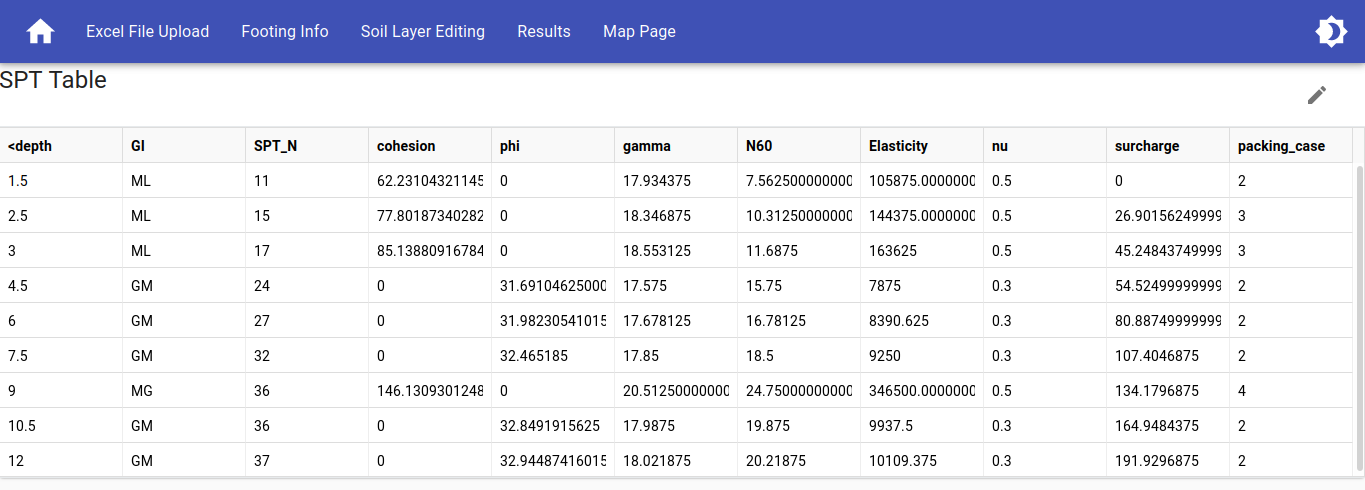
\includegraphics[width=\linewidth,keepaspectratio]{../proj/soilbearing/media/images/preview_mode.png}
See program internal interpolations, etc. \\

\subsection{Results Tab}
There are 2 options:-\\
\subsubsection{From datas as above}
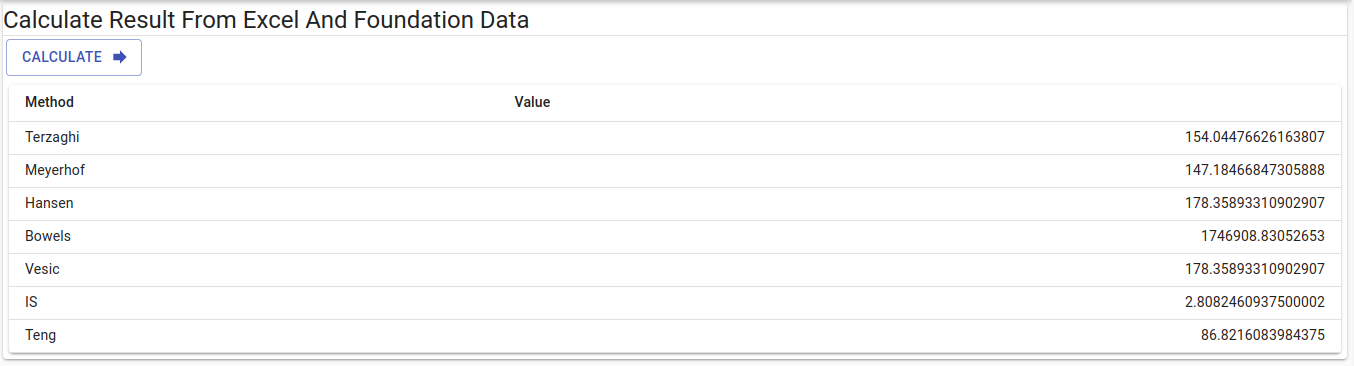
\includegraphics[width=\linewidth,keepaspectratio]{../proj/soilbearing/media/images/fed.png}
Calculation as per above datas.\\

\subsubsection{Calculate from Interpolation}
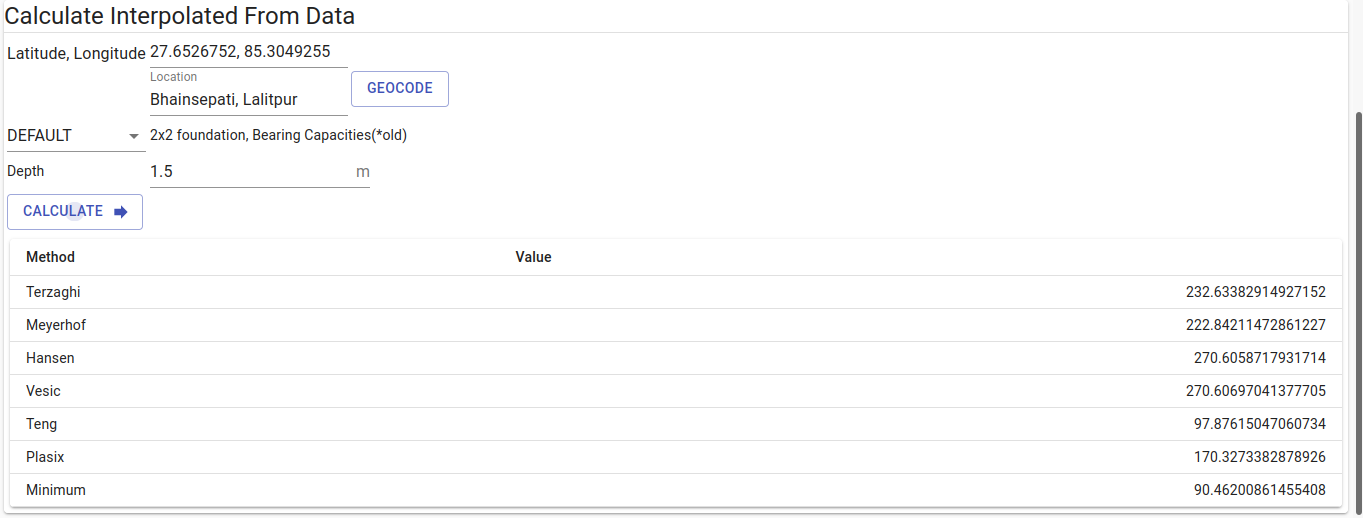
\includegraphics[width=\linewidth,keepaspectratio]{../proj/soilbearing/media/images/ID.png}
Datas interpolated by IDW from the project report datas.\\
Geocode from name, to get latitude and longitude.\\

\subsection{Map Tab}
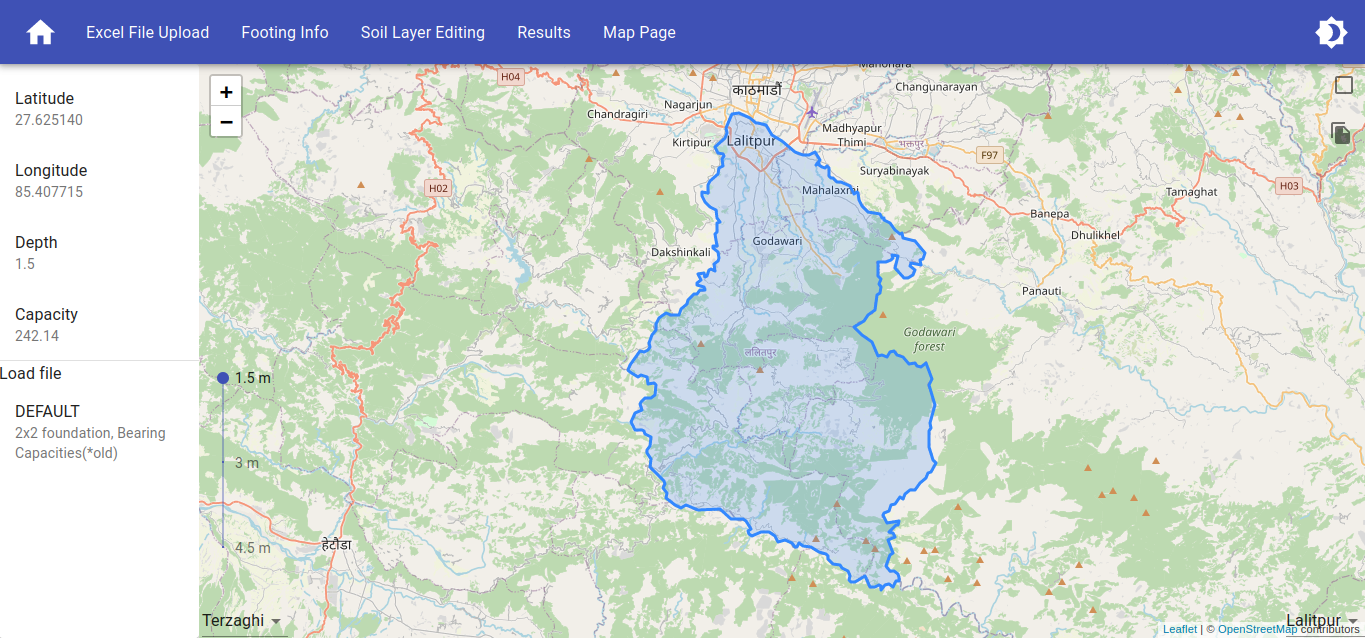
\includegraphics[width=\linewidth,keepaspectratio]{../proj/soilbearing/media/images/map_page.png}
Map from datas computed by interpolation.